\documentclass[man,floatsintext]{apa6}
\usepackage[nodoi]{apacite}
\usepackage{graphicx}
\usepackage[american]{babel}
\usepackage{amsmath}
\usepackage{enumitem}
\title{Beyond Na\"{i}ve Cue Combination: Salience and Social Cues in Early Word Learning}
\author{Daniel Yurovsky and Michael C. Frank}
\affiliation{Department of Psychology, Stanford University}
\shorttitle{Cue Combination}
\leftheader{Yurovsky \& Frank}

\abstract{Children learn their earliest words through social \emph{interaction}, but it is unknown how much they rely on social \emph{information}. Some theories argue that word learning is fundamentally social from its outset, with even the youngest infants understanding intentions and using them to infer a social partner's target of reference. In contrast, other theories argue that early word learning is largely a perceptual process in which young children map words onto salient objects. One way of unifying these accounts is to model word learning as weighted cue-combination in which children attend to many potential cues to reference, but only gradually learn the correct weight to assign each cue. We tested 3 predictions of a na\"{i}ve cue-combination account using an eye-tracking paradigm that combines social word-teaching and two-alternative forced-choice testing. None of the predictions were supported. Thus, while aspects of this unifying account are correct, it must be amended to capture the dynamics of children's behavior across differing referential situations. In addition, we discuss methodological implications for research using two-alternative displays. }

\keywords{Language acquisition, word learning, attention, social cues, eye-tracking, cognitive development}

\authornote{Please address correspondence to: 

\vspace{12 pt}
Daniel Yurovsky

Jordan Hall (Building 420)

Stanford University

450 Serra Mall

Stanford, CA 94305

\vspace{12 pt}
Email: yurovsky@stanford.edu 
}

\begin{document}
\maketitle


How do children learn the meanings of their first words? A number of influential theories conceptualize young infants' primary learning mechanism as making associations between perceptual stimuli \cite{Piaget1952, Vygotsky1978}. On these kinds of accounts, infants learn the meanings of labels like ``ball'' and ``dog'' by mapping them onto salient objects in their learning environments \cite{Werker1998,Smith2000}. These accounts are appealing on grounds of parsimony: the mechanisms they require for the onset of word learning---perceptual orienting and associative mapping---are universally agreed to be in the repertoire of young infants (\citeNP<e.g.>{Fantz1964,Haith1980}; although \citeNP<c.f.>{Spelke1998}). In addition, the ecological context of language learning appears to support perceptually-driven learning. For instance, early child-directed naming events are characterized by multi-modal synchrony: mothers move the objects they label in temporal synchrony with the labels they speak \cite{Gogate2000}, and the degree of synchrony predicts successful word-object mapping for young infants \cite{Gogate2006}.\footnote{For convenience here---and reflecting the orientation of our work towards concrete noun learning---we refer to ``word-object mapping'' and ``word learning'' interchangeably. Of course, mapping is only a small part of the process of learning a word, which includes at least: learning a phonological form, mapping this form to a referent, inferring the meaning that licenses this reference and how it generalizes across instances, and retaining all of this information in memory for future use.}

Infants are also situated in a social system from their first day of life, however. This social system is the \emph{source} of the multi-modal structures in their perceptual input. Alternative theories thus argue that infants leverage social---not just perceptual---information when learning even their first words \cite{Bruner1983,Bloom1998}. For instance, infants follow direction of gaze by 6-months \cite{Dentremont1997}, especially in the presence of other communicative signals \cite{Senju2008}, and individual differences in gaze-following predict differences in vocabulary development \cite{Brooks2008}. In addition, in some experiments infants appear to be representing others' beliefs, and these representations affect their expectations by 12 or even 6 months of age (\citeNP{Vouloumanos2012, Vouloumanos2014}; cf. \citeNP{heyes2014}). Infants are thus tuned to social cues, and could in principle already use these cues from the outset of word learning.

Because these two classes of theories are posed as mutually-exclusive competitors, and because both are supported by compelling empirical findings, each has attempted to re-conceptualize the evidence in favor of the other on its own terms. For example, researchers in the perceptual tradition have shown that cases of putatively social understanding can be explained as a set of learned perceptual associations \cite<e.g.>{Goldstein2008, Yu2012c, Deak2014}. On the other side, researchers from the social tradition have argued that the perceptual signals shown to drive learning are effective \emph{because} infants infer that they are being presented by a social, pedagogically motivated caregiver \cite{Csibra2010, Deligianni2011}. 

Unifying these two accounts within a single framework provides a promising theoretical alternative. As advocates of social word learning point out, children must learn more than mappings between labels and objects in the world. While object labels represent a large slice of typical early vocabularies \cite{Caselli1995,Tardif2008}, young children also learn verbs, adjectives, and many other word types \cite{Fenson1994,Clark2003,Bergelson2013}. It is likely that the kinds of mechanisms advanced in perceptual accounts of early word learning are not completely sufficient to explain this diversity of word meanings \cite{Gleitman1990,Bloom2000,Waxman2009}, despite work showing that these mechanisms do play a role \cite{Piantadosi2012,Scott2012}. While we focus here on concrete noun learning, the scalability of learning mechanisms to the broader vocabulary is an important theoretical concern for unifying models.

One possible proposal for unification is that infants are sensitive to many cues to reference: both perceptual cues like visual salience and temporal contiguity \emph{and} social cues like eye-gaze and pointing. To determine the referent of a speaker's utterance, children could combine all of the available cues, assigning each a weight proportional to its predictive validity. On such an account, developmental changes in determining a speaker's target of reference are due to a process of learning the correct weights to assign to each kind of cue. Early on, children may be biased to assign high weight to perceptual cues. However, over development, children might gradually assign higher weight to social cues as they learn that they are better predictors of reference \cite{Hollich2000, Golinkoff2006}. The goal of our current work is to test this kind of unifying ``developmental cue combination'' account; we begin by reviewing previous research supportive of such an account and then derive several predictions, which we test in two experiments. 

\subsection{Data Supporting Developmental Cue Combination}

The primary support for a developmental cue-combination account comes from studies that pit perceptual salience against social information (e.g., speaker gaze) and measure children's learning under these conditions at different ages. \citeA{Hollich2000} presented 12 studies that varied the referential cues highlighting two different objects in ambiguous naming events. In the first three experiments, one of the objects was perceptually salient, and one was fixated by the speaker. Analyses compared a condition in which the same object received both cues (Coincidental) to a condition in which the cues pointed to different objects (Conflict). In these studies, 19- and 24-month-olds appeared to assign more weight to the social cue, preferentially mapping the label onto the object the speaker fixated regardless of which was more salient. In contrast, although 12-month-olds showed some evidence of following the speaker's gaze in training, they looked more at the more salient object at test in both conditions. A followup experiment from \citeA{Pruden2006} showed that 10-month olds did not attend to the speaker's gaze at all.

In almost all of these studies, however, target and competitor objects remained in the same position during both training and test. Thus, it is unclear in most of this data whether infants mapped the label onto an object or onto a location \cite<e.g.,>{Benitez2012}. In the two experiments in which target position switched from training to test, learning was disrupted for all of the age groups except the 24-month-olds \cite{Hollich2000, Pruden2006}. This finding is consonant with earlier data  showing in a head-turn procedure that conflicting perceptual and social cues disrupted learning in 18- but not 24-month-olds \cite{Moore1999}. 

Together, these studies present data that are supportive of a developmental cue combination account, but the data are incomplete for a number of reasons. First, previous experiments only measured infants' accuracies at test. Without measurements of how cues affect attention during training, it is unknown why manipulations of salience or social cues had different effects for different age groups. In particular, it could have been the case that salience had differential effects on children's looking behavior at test time than at training, regardless of their sensitivity to social cues (a situation we show to be the case for our data). Second, it is unclear from prior work whether changes in the relative strengths of social and perceptual cues would be due to increasing weights for social cues, decreasing weights for perceptual cues, or both. Answering this question would require comparing conditions where cues are in opposition to a condition where \emph{only} the social cue is available.\footnote{While \citeA{Moore1999} did compare these conditions, they have relatively low power to detect differences between them due to small samples and a challenging test measure (forced choice responding). \citeA{Hollich2000} ran studies using gaze alone with 12-month-olds, but not with older age groups.} The goal of our current studies is thus to gather a large, developmentally-broad eye-tracking dataset on children's behavior in cue-combination tasks, both during training and at test. This dataset allows us to make a direct test of predictions of the developmental cue combination account, which in turn addresses these questions.

% these studies do not link children's behavior during training trials to their outcomes at test. Because these studies did not track children's eye-gaze, they do not capture the dynamics of attention in the presence of different cues to reference. That is, they characterize children's preference for one object over the other, but not how children allocated their attention to the speaker and toys over time. 

\subsection{Testing Predictions of Developmental Cue Combination: The Current Study}

Weighted cue-combination is an intuitive, computationally simple model of the process of change in early word learning. For example, a number of computational models have implemented a version of this idea  \cite{Frank2007b,Frank2013a}. This model is also consistent with properties of our perceptual system: Within and across modalities, adults weigh cues in proportion to their predictive power, combining them as predicted by ideal observer models \cite{Ernst2002, Jacobs2002}. Despite this intuitive plausibility, a number of detailed predictions of cue combination models remain untested, specifically as they apply to these models as a description of developmental change in children's concrete noun learning. 

In the current study, we test three predictions of the cue-combination model of developmental change:

\begin{enumerate}[noitemsep]
	\item Developmental change is due to re-weighting across cues,
	\item Perceptual cues decrease in weight across early development, 
        \item Social cues increase in weight across early development, and
	\item Cue weights drive attention during learning.
\end{enumerate}

\noindent Prediction \#1 is derived directly from previous work, which suggested that a major developmental change during the second year was a move from reliance on salience to reliance on social cues. The developmental cue combination account predicts that this shift should be a major driver of developmental change in word learning during this period. Predictions \#2 and \#3 are corollaries of Prediction \#1, again following from previous work that suggested that perceptual cues were less relevant for older children and that their learning was driven more by social cues. Finally, Prediction \#4 comes from the idea that cue combination affects learning through the biasing of attention during word learning; thus, greater cue weights on social cues relative to salience should be reflected by shifts in the distribution of gaze when these two cues are in conflict. 

In two experiments, we show that none of these predictions is supported. Thus, while cue-combination captures important insights about early word learning, a na\"{i}ve version of this account is insufficient to explain the observed developmental trajectory. We end by discussing possible modifications to this view.

\section{Experiment 1}

In nearly all previous experiments investigating cue-combination in early word learning, social cues were pitted against perceptual cues \cite<c.f.>{Moore1999}. Thus, results indicating developing preferences for social information over perceptual information are consistent with three possible explanations: (1) social cues increase in weight, (2) perceptual cues decrease in weight, or (3) perceptual and Social Cues both change in their \emph{relative} weight. Experiment 1 was designed to distinguish between these three possibilities by independently measuring the development of children's abilities both to follow and to learn from social gaze, in the \emph{absence of competing salience cues}. A na\"{i}ve cue-combination account, in which developmental changes in cue use result from learning their relative predictive weights, makes a null prediction: Children's responses should not change significantly across development when only one cue is available. 

We tracked children's eye movements while they watched a series of naturalistic word-learning videos. In each, children saw a speaker seated at a table between two novel toys. She greeted them, and then turned towards one of the toys and labeled it three times in a short monologue. After these learning trials, children were tested for their knowledge of the referent for the new word using the preferential looking procedure. In addition, to measure children's processing abilities for familiar words, similar test trials were administered with known items.

\subsection{Method}

\begin{figure}[tb]
	\center{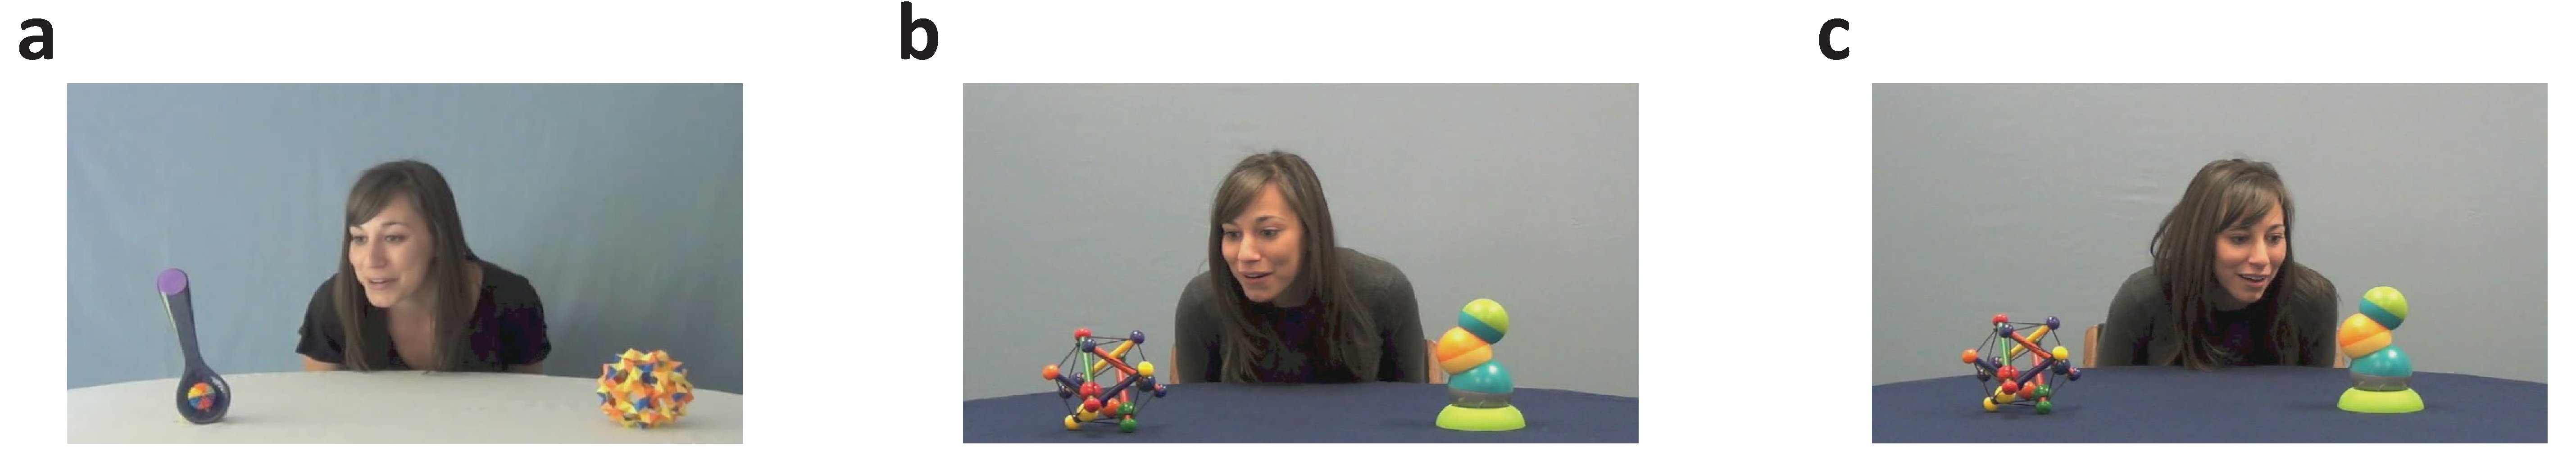
\includegraphics[width=\textwidth]{figures/tri_fig.pdf}}
	\caption{\label{fig:design} Example learning trials from Experiments 1 and 2. In Experiment 1 (a), the speaker turned towards one of the equally-salient toys and labeled it three times over the course of $\sim$10 seconds. In Experiment 2, the speaker produced the same social cues and the same label as in Experiment 1, but the target object was either the more perceptually salient toy (b), or the less perceptually salient toy (c). These manipulations allowed us to measure the contributions of both salience and social information to word-object mapping.}
\end{figure}

\subsubsection{Stimulus Norming}
To minimize salience differences between the two potential referents, we first normed them using aggregate adult judgments. Thirty-eight adults on Amazon Mechanical Turk were shown toys two at a time from a set of 10. For each pair, they were asked to pick the toy they would rather play with. Each participant made 20 choices, with toys sampled at random, producing $\sim$7.6 responses for each pair of toys. Based on these responses, we selected the two toys that were best balanced against each other (see Figure~\ref{fig:design}a).

\subsubsection{Participants}

Parents and their 1--4 year-old children were invited to participate in a short language learning study during their visit to the San Jose Children's Discovery museum. In total, we collected demographic and experimental data from 269 children, 122 of whom were excluded for one or more of the following reasons: abnormal developmental issues ($N= 27$), failure to calibrate ($N=58$), and less than 75\% exposure to English ($N=36$).\footnote{These exclusion criteria were preset in this study on the basis of previous work \cite{Yurovsky2013c}.} The final sample consisted of 27 1--1.5 year olds (9 girls), 19 1.5--2 year olds (7 girls), 38 2--2.5 year olds (13 girls), 26 2.5--3 year olds (10 girls), 15 4--3.5 year olds (9 girls), and 22 3.5--4 year olds (11 girls).

\subsubsection{Stimuli and Design}

The experiment consisted of two kinds of trials designed to measure both how children allocate their attention while learning from a social partner, and what word-object mapping information they extract from these learning events. Learning trials were $\sim$12s video clips in which a speaker first greeted the the child, and then turned towards one of the two toys on the screen, labeling it three times in a short monologue (Figure~\ref{fig:design}a). On the first learning trial, for example, the speaker said ``Hi there! It's a \emph{modi}. Look at the \emph{modi}. What a nice \emph{modi}.''

On each test trial, children saw two objects---one on each side of the screen---and heard a short audio clip of the speaker from the learning trials asking them to find a target object. Each test trial was 7s long, and the target label was heard at ~2.75s. On \emph{Familiar} test trials, both the target and competitor were common objects familiar to young children (e.g. book vs. dog). On \emph{Novel} and  \emph{Mutual Exclusivity (ME)} test trials, children saw both of the toys from the previous learning trials, and were asked to find either the previously named toy (\emph{modi}), or were asked about a novel label (\emph{dax}). These ME trials were designed as a strong test of mapping formation. Looking to the correct target on Novel trials alone could result from familiarity or preference rather than mapping, but correct performance on both Novel and ME trials could only result from knowledge of the specific label used in training.

Finally, the experiment contained two calibration checks: short videos in which small dancing stars appeared in four places on the screen. These checks allowed us to adjust initial calibration settings when they were imprecise \cite<for details of this procedure, see>{Frank2012d}.

\subsubsection{Procedure}

The eye-tracker was first calibrated for each child using a 2-point calibration. Next, children saw four learning trials in which the speaker looked at one of two toys on the screen and labeled it three times. Finally, children saw the test trials, in which their knowledge of both familiar and novel word-object mappings was tested. Two calibration checks (described above) were embedded in the learning phase. The entire experiment consisted of 4 learning trials, 8 Familiar, 6 Novel, and 6 ME test trials.

\subsection{Results}

We begin by describing children's behavior during both training and test trials before moving on to discussing its implications for the predictions of the developmental cue combination model. We analyzed children's eye movements using a Region of Interest (ROI) approach. Bounding-box ROIs were drawn by a human coder for the speaker's face (learning trials) and for the two objects (learning and test trials). Children's learning and test behaviors were quantified by measuring their proportion of looking to each ROI on each trial. To ensure that proportions were representative, individual test trials were excluded from analysis if eye gaze data were missing for more than half of their duration. To compute age-group looking proportions, proportions were computed first for each individual trial, averaged at the individual-child level, and then averaged across children.



To ensure accuracy in our identification of point of gaze, children's calibrations were adjusted by fitting a robust linear regression for their fixations relative to known locations on calibration check videos. These regressions were used to transform eye movements for all learning and test trials \cite{Frank2012d}.


Window-of-analysis selection began by coding the point of disambiguation for each trial. This was the onset of the target label for test trials, and the rotation of the speaker's head for learning trials. The window for each trial began 1s after this point of disambiguation to allow children of all ages enough time to process and continued out to 3s after this point on both learning and test trials. To quantify learning with standard analyses, we aggregated these patterns of looking over time to compute proportion of target looking on each test trial. JUSTIFY WINDOW CHOICE?




First, children were broadly 

I THINK WE NEED TO DISCUSS THE RESULTS PER SE BEFORE TESTING PREDICTIONS IN THIS LONGER FORM PAPER.

E.G. SHOW TRAINING ROI CURVES THAT WE CUT FROM THE COGSCI PAPER?

ALSO RECOGNITION CURVES FOR FAMILIAR, NOVEL, ME - SO CAN BE COMPARED WITH PRIOR WORK AND SO WE CAN SEE WHAT'S GOING ON WITH YOUNGEST KIDS.

\begin{figure}[tb]
	\center{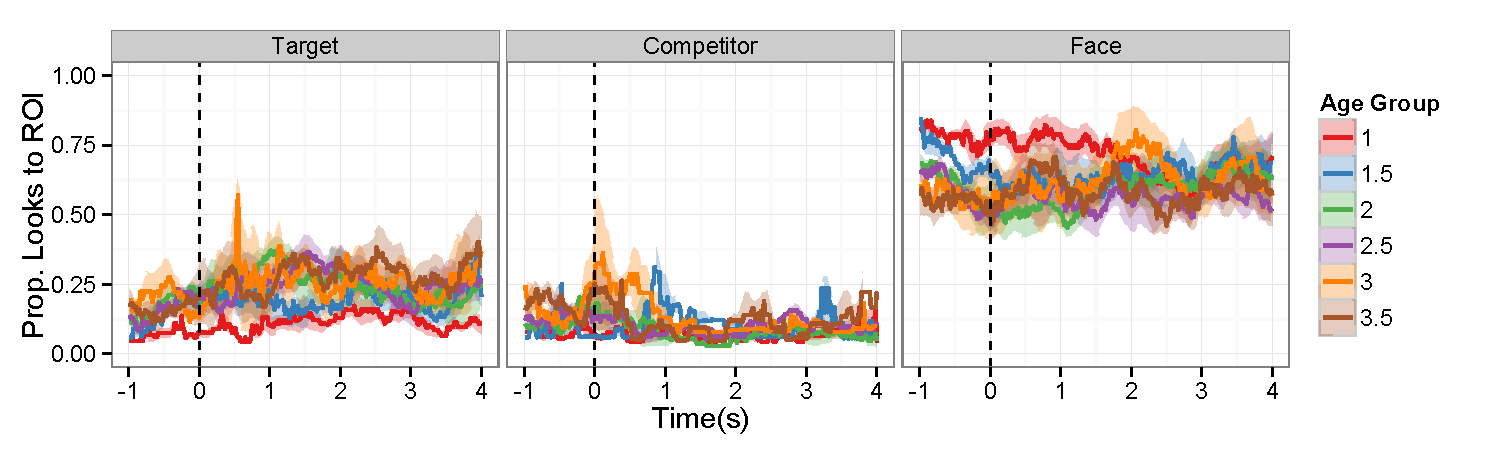
\includegraphics[width=\textwidth]{figures/exp1_train_spaghetti.pdf}}
	\caption{\label{fig:design} Looking behavior during training trials in Experiment 1. Children in all age groups spent the majority of training trials fixating the speaker's face.}
\end{figure}

In Experiment 1, we address two predictions of na\"{i}ve cue combination: how cues affect attention during learning, and how weights change across development.

\subsubsection{Older children were better at \emph{disengaging} from social stimul} 

Children were successful at attending to and following the speaker's social gaze even from the youngest ages measured. Children of all ages spent more time looking at the target than at the competitor during learning trials (smallest $t(23)  = 3.20$, $p < .01$; Figure~\ref{fig:exp1_train_test}). However, for all age groups, looks to both target and competitor made up the minority of children's dwell times. Instead, children in all age groups spent more than 50\% of their time attending to the speaker's face (Figure~\ref{fig:exp1_train}).\footnote{All data and code for analysis available at \small{\tt{http://github.com/dyurovsky/ATT-WORD}}.} Thus, the primary driver of developmental change was not stronger discrimination between the target and competitor (predicted by greater social cue weights), but rather improved ability to disengage from the speaker's face. 

 \begin{figure}[tb]
	\center{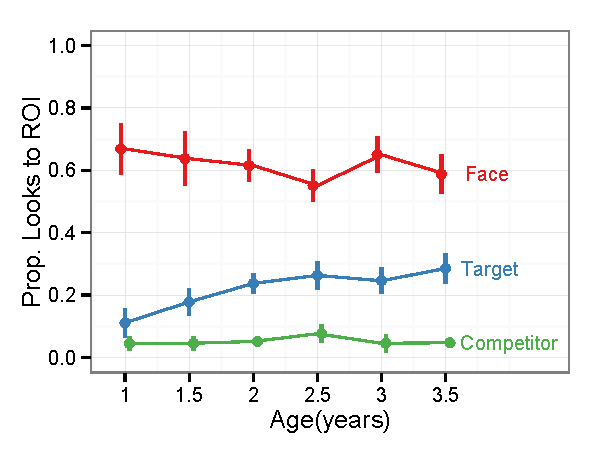
\includegraphics[width=.65\textwidth]{figures/exp1_train.pdf}}
	\caption{\label{fig:exp1_train} Proportion of children's looking the target toy, competitor toy, and the speaker's face during learning in Experiment 1. Children of all ages spent the majority of the learning trials looking at the speaker's face. Disengaging from the face and fixating the target increased across development. Error bars indicate 95\% confidence interval computed by non-parametric bootstrap.}
\end{figure}

\vspace{9 pt}

\subsubsection{Developmental change was not primarily due to re-weighting} 

In line with the na\"i{v}e cue combination account, attention due to the social cue during learning carried forward to correct mapping at test. Analyses of test trials showed broad success on Familiar, Novel, and ME trials across development. The 1--1.5 year-olds trended towards significance on familiar trials ($t(26)  = 1.65$, $p = .11$), and were non-significantly in the correct direction on Novel and ME trials. At all other ages, children looked to the target at above-chance levels on all test trials (smallest $t(17)  = 2.10$, $p = .05$). 

However, children's abilities both to follow social cues during learning trials and to find the correct target on test trials improved across development. To quantify this improvement, we fit a mixed effects logistic regression to the data \cite{Jaeger2008}. This analysis revealed significant improvement across age ($\beta = .61$, $z = 4.03$, $p <.001$), as well as a significant significant effect of Learning as compared to Novel trials ($\beta = 1.18$, $z = 3.11$, $p <.01$). No other effects or interactions approached significance. Figure~\ref{fig:exp1_train_test} shows proportion of looking to the correct target for all kinds of trials at all ages. 

Thus, across development, children improved in learning from the social cue, even when it was the only cue available. This suggests that relative re-weighting across cues is not the only driver of improved word learning.

\begin{figure}[tb]
	\center{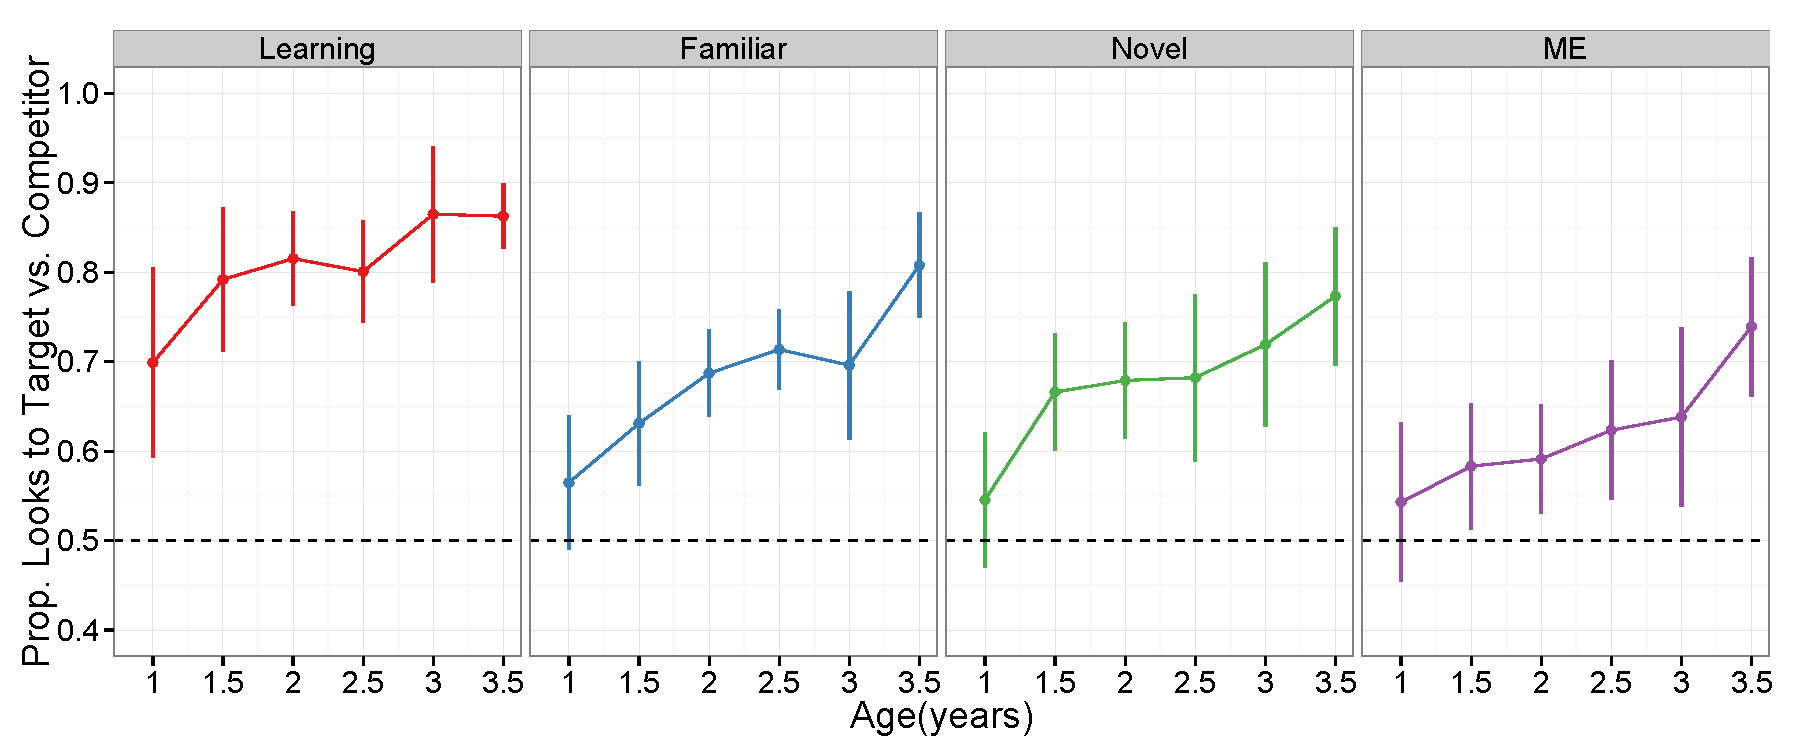
\includegraphics[width=.65\textwidth]{figures/exp1_train_test.pdf}}
	\caption{\label{fig:exp1_train_test} Proportion of time children fixated the correct target on each type of test trial in Experiment 1. Children improved on all measures across development. Each dot indicates one half-year age group and each line represents a 95\% confidence interval computed by non-parametric bootstrap. A proportion of .5 indicates chance performance.}
\end{figure}	

\subsection{Discussion}

Together, these results provide evidence both of early competence in the use of social gaze to determine the target of a speaker's reference, as well as improvement across development. Further, improvements in gaze-following also paralleled improvements in both finding the referents of these novel words on subsequent test trials, and also finding the referents of familiar words (Figure~\ref{fig:exp1_train_test}).

These results thus provide support for one key claim of the developmental cue-combination account: children are sensitive to social cues quite early. Young children could assign small---but non-zero---weight to social cues, and then gradually assign them more weight over development. However, the results also provide evidence \emph{against} the predictions that cues drive attention, and that developmental change is due to relative re-weighting. First, children of all ages found the speaker's face highly engaging, and spent the majority of their time fixating it rather than the referents on learning trials. The primary behavioral development was the ability to {\it disengage} from the speaker's face. Second, children showed gradual improvement in fixating the target during both learning and test trials well into their fourth year.

This data could be consistent with a modified version of the cue-combination account in which cues change in both their absolute and relative weights due to learning. However, while children undeniably encounter naming events in their third and fourth years, it seems unlikely that the process of learning the validity of social gaze would extend over such a long period of time. 

TRANSITION?

In Experiment 2 we manipulated the relative salience of the target and competitor objects children learned about \cite<c.f.>{Hollich2000}. This allowed us to measure how salience affects children's looking during both learning and test, providing a test of all three predictions of the na\"{i}ve cue-combination account.

\section{Experiment 2}

Experiment 2 was identical to Experiment 1 in all respects except for the identity of the novel toys that served as the target and competitor. In contrast to Experiment 1, in which the two toys were balanced in their visual salience, the two toys in Experiment 2 were mismatched. For children in the \emph{Salient} condition, the target was the more interesting toy, and the competitor the less interesting toy. In the \emph{Non-Salient} condition, the identities of the toys were switched---the target was the less salient toy. Experiment 2 allowed us to investigate children's use of social cues to learn new words both social cues and salience indicate the same referent, and when they are in competition \cite<as in>{Hollich2000,Pruden2006}.

\subsection{Method}

\subsubsection{Participants}

Participants were recruited from the floor of the San Jose Children's Discovery museum as in Experiment 1. For Experiment 2, we focused on the three youngest age groups. In the Salient condition, demographic and experimental data were collected from 117 children, 52 of whom were excluded for one or more of the following reasons: abnormal developmental issues ($N= 13$), failure to calibrate ($N=25$), less than 75\% exposure to English ($N=33$), and inattentiveness ($N=2$). The final sample consisted of 22 1-1.5 year olds (11 girls), 21 1.5-2 year olds (10 girls), 19 2-2.5 year olds (9 girls). 

In the Non-Salient condition, data were collected from 126 children, 71 of whom were excluded for one or more of the following reasons: abnormal developmental issues ($N= 9$), failure to calibrate ($N=26$), and less than 75\% exposure to English ($N=36$). The final sample consisted of 26 1-1.5 year olds (13 girls), 25 1.5-2 year olds (11 girls), 15 2-2.5 year olds (4 girls).

\subsubsection{Stimuli, Design, and Procedure}

Experimental stimuli were identical to those in Experiment 1, except that the identities of the novel toys were changed and new videos were recorded. The procedure, including the order of the trials, was identical.

\subsection{Results and Discussion}

\begin{figure}[!h]
	\center{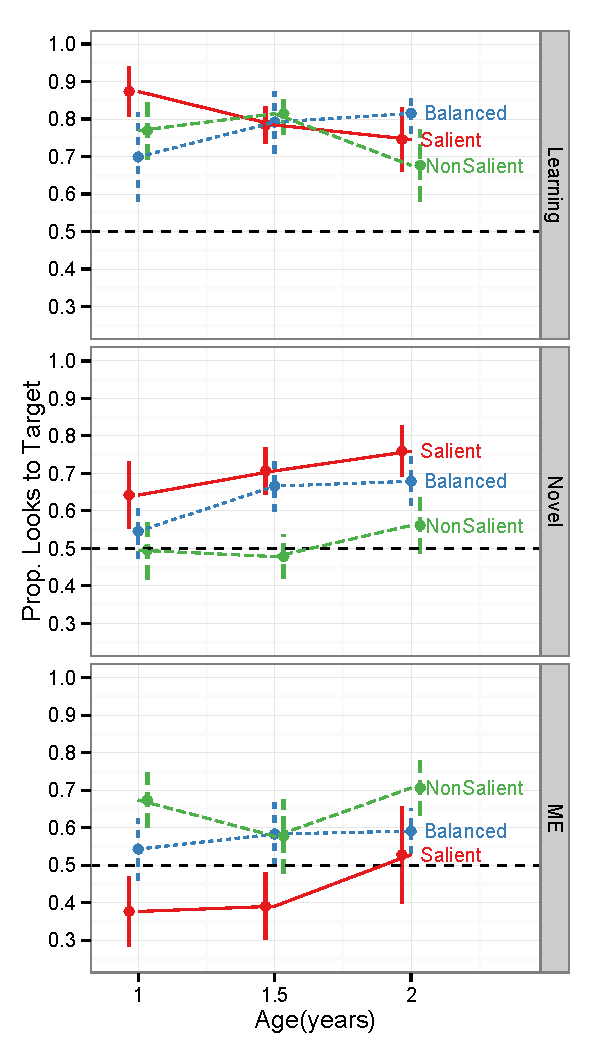
\includegraphics[width=.6\textwidth]{figures/exp1_2_train_test.pdf}}
	\caption{\label{fig:exp1_2} Proportion of time children fixated the correct target on Learning and Test trials in Experiments 1 (three youngest age groups) and 2. Salience had the predicted effect on looking behavior at test, but relatively little during learning. Each dot indicates one half-year age group and each error bar represents a 95\% confidence interval computed by non-parametric bootstrap. A proportion of .5 indicates chance performance.}
\end{figure}


AGAIN, NEED BASIC DESCRIPTIVE ANALYSES: WERE PARTICIPANTS ABOVE CHANCE? WHAT DID THEY LOOK AT, ETC...

To determine the effect of perceptual salience on word learning, we compared children's looking in the Salient and Non-Salient conditions not only to each other, but also to the Balanced condition tested in Experiment 1. 

\subsubsection{Perceptual salience did not drive attention during learning} 

In contrast to the prediction of the na\"{i}ve cue-combination account, children's looking behavior during learning trials was not significantly affected by the salience of the target and competitor (Figure~\ref{fig:exp1_2}, top). As in Experiment 1, children of all ages spent the more time looking at the target than the competitor, but looking time to both made up the minority of their dwell time; children spent the majority of learning trials looking at the speaker's face (smallest proportion---2-year-olds in the Non-Salient Condition: .51).

This null-result could be due to the toys being too similar in their salience, making this a weak test of the cue-combination model. However, salience exerted a strong effect on test trials---children in all age groups were strongly attracted to the salient object. When the target referent was salient, children at all ages looked at it for the majority of the window of analysis on Novel test trials (smallest $t(19)  = 2.96$, $p < .01$). When the target was non-salient, no age group look showed evidence of learning on Novel test trials (largest $t(13)  = 1.46$, $p = .17$). Mutual-exclusivity (ME) trials showed the opposite pattern. When the target referent was salient, children in the two younger age groups looked at the correct referent on ME trials (the competitor) at \emph{below} chance levels (smallest $t(20) = -2.29$, $p < .05$). In the Non-Salient condition, even the youngest children looked at the correct referent on ME trials at above chance levels (smallest $t(22) = 4.51$, $p < .001$). Figure~\ref{fig:exp1_2} (middle and bottom) shows looking behavior at test in both Experiments 1 and 2.


\begin{table}[!t]
\centering
\caption{Mixed-effects Logistic Regression Model for Looking Behavior in Experiments 1 and 2.} 
\label{tab:model_table}
\begin{tabular}{lrrrrl}
 Predictor & Estimate & Std. Error & $z$ value & $p$ value &  \\ 
  \hline
Intercept & -0.63 & 0.63 & -0.99 & 0.32 &  \\ 
  Age(years) & 0.43 & 0.27 & 1.61 & 0.11 &  \\ 
  Familiar & 1.53 & 0.73 & 2.10 & 0.04 & * \\ 
  Salient & 0.92 & 0.48 & 1.90 & 0.06 & . \\ 
  NonSalient & -1.00 & 0.37 & -2.70 & 0.01 & ** \\ 
  Learning & 0.94 & 0.44 & 2.11 & 0.03 & * \\ 
  ME & -0.32 & 0.36 & -0.89 & 0.37 &  \\ 
  Salient $\times$ Learning & 0.00 & 0.84 & 0.00 & 1.00 &  \\ 
  Non-Salient $\times$ Learning & 1.15 & 0.65 & 1.76 & 0.08 & . \\ 
  Salient $\times$ ME & -2.23 & 0.61 & -3.65 & 0.00 & *** \\ 
  Non-Salient $\times$ ME & 1.59 & 0.54 & 2.92 & 0.00 & ** \\ 
   \hline
\end{tabular}
\end{table}
\subsubsection{Perceptual cues did not decrease in weight across development}

The effect of perceptual cues at test did not appear to change across the 1--2 year range. We fit a mixed-effects logistic regression to the data from both experiments to determine how age and experimental condition impacted looking behavior during both learning and test. After controlling for performance on Familiar trials, this regression showed a significant effect of condition, and an interaction between trial type and condition. Children looked more to the salient object at test regardless of whether it was the target or competitor, and significantly more at the target during learning trials regardless of whether it was salient. None of these factors interacted with age (Table~\ref{tab:model_table}). 

\subsubsection{Developmental change was not due to re-weighting across cues} 

Together with the t-tests above, the mixed-effects model suggests that children are not relatively re-weighing salience and social cues over the course of development. While salience certainly plays a role in directing looking behavior, it does not appear to play a role during learning itself. However, salience has a strong effect during test: In the absence of any social information, salience directs children's attention in a way that does not appear to change over early development.

\section{General Discussion}

Is children's early word-object mapping fundamentally social, or is it mostly driven by perceptual processes? A weighted cue-combination account provides a simple framework to unify social and perceptual factors in early word learning \cite{Hollich2000, Frank2013a}. Under this kind of account, perceptual cues are weighed higher in early learning, while social cues gradually gain weight as children learn their predictive power across early naming events. We tested this account in two word-learning experiments and found that its predictions were inconsistent with the data. 

Although a na\"{i}ve cue-combination account would predict that developmental change is largely driven by the relative re-weighting of cues, our data showed little evidence of this (contra prediction 1). Instead, developmental changes during learning appeared to be driven by disengagement from the social stimulus, not disengagement from the perceptually salient target (contra prediction 2). Finally, perceptual salience exerted its effects mostly at test, and did so consistently across early development instead of decreasing in weight (contra prediction 3).

These results present a picture of early word learning that is consistent with the spirit of cue-combination accounts like the Emergentist Coalition model, but which requires significant refinement of their details. For instance, although perceptually salient toys may attract attention and direct looking and learning in the absence of social partners, the speaker herself was the most interesting aspect of our naming events for young children. Although it is unclear to what extent young children's attention to the speaker reflects their understanding of her intentions, it is quite clear that their attention was both attracted and directed by social information. The primary change in cue-use across development may thus be due decreasing weight on perceptually salient toys, but rather to developing inhibitory control more broadly.

NEW PARAGRAPH: ONLY OK. Our work here has significant implications for users of two-alternative preferential looking displays. We found that, when alternatives were not matched for perceptual salience, the relatively more salient object dominated children's looking preferences for all age groups. In particular, we saw evidence of novel word learning for the 1.5--2-year-olds in the balanced salience condition, but this result was masked if the target item was more salient and exaggerated if the target was less salient. Especially for these young participants, small differences in the perceptual properties of the stimuli may mask learning, presumably because overcoming perceptual salience requires inhibitory control that these young children do not have. \citeA{fernald2008} discusses the utility of matching displays for salience in order to achieve precise measurements with young children. Our dat ratify this suggestion and suggest that such matching is especially important when comparing across ages, since children's changing inhibitory capacities would otherwise pose a confound in interpreting changes in looking.

COULD BE INTERESTING TO LOOK AT WHETHER THE AVERAGE OF SALIENT AND NON SALIENT IS DIFFERENT AT ALL FROM BALANCED?

Learning a new word relies on processes that work at multiple time-scales. Children need to identify a speaker's referent in-the-moment, encode a mapping between the label and referent, recall multiple labeling events and integrate acrobatss them, and use their learned mappings to identify the object in novel contexts \cite{Frank2009a,McMurray2012, Yu2012b}. We have provided data here that falsify some predictions of a na\"ive cue-combination model. But our critiques converge with a broader theoretical problem: na\"{i}ve cue-combination does not distinguish among the component problems that word learners must solve. In our experiments, for instance, children used different cues to identify a speaker's referent and to find it in a novel test context. Building a more satisfying model of the development of word learning will require integrating the cues children use to identify referents with an understanding of how these cues interact with attentional control, memory, and the conversational contexts in which naming occurs \cite{Frank2013a, Yurovsky2013c}.

\section{Acknowledgments}

We are grateful to Janelle Klaas for collecting the data, and to  all of the members of the Language and Cognition Lab for their feedback on this project. In addition, we thank the parents, children, and staff at the San Jose Children's Discovery Museum for supporting us in collecting developmental data. This work was supported by NIH NRSA F32HD075577 to DY as well as grants from the Merck Scholars Foundation and the Stanford Center Health Research Initiative to MCF.

\bibliographystyle{apacite}
\bibliography{library12}

\end{document}
